\section{Proxy and API Layer}

\subsection{ProxyState Component Container}

The \texttt{ProxyState} is the central container that holds all shared components for a Nexa-Proxy instance. It implements the ``composition root'' pattern from dependency injection literature---a single struct that owns all subsystem references and provides them to handlers:

\begin{lstlisting}[language=Rust, caption={ProxyState struct definition.}]
pub struct ProxyState {
    pub did_resolver: DIDResolver,
    pub capability_registry: CapabilityRegistry,
    pub semantic_router: SemanticRouter,
    pub channel_manager: ChannelManager,
    pub budget_controller: BudgetController,
    pub security_manager: SecurityManager,
    pub storage: MemoryStore,
    pub config: ProxyConfig,
}
\end{lstlisting}

Each field is an Arc-wrapped shared reference, enabling concurrent access from multiple HTTP handler tasks within the Tokio~\cite{tokio2022} async runtime. The \texttt{ProxyState::new()} constructor initializes all components with default configuration, while \texttt{ProxyState::with\_config()} allows customization via the \texttt{nexa-proxy.toml} file.

The ProxyState is injected into all REST API handlers through Axum's~\cite{axum2022} state extraction mechanism: \texttt{axum::extract::State<ProxyState>}. This pattern ensures that every handler receives the same shared state without global variables or manual thread-safety management.

\subsection{REST API: 7 Endpoint Design}

The REST API provides an HTTP interface for agents that cannot use the binary RPC protocol directly. Seven endpoints cover the essential proxy operations:

\begin{table}[h]
\centering
\begin{tabular}{@{}llll@{}}
\toprule
Endpoint & Method & Function & Mean Latency \\
\midrule
/v1/health & GET & Health check (no state) & 1.202\textit{ms} \\
/v1/register & POST & Register capability & 1.270\textit{ms} \\
/v1/discover & POST & Semantic discovery & 1.449\textit{ms} \\
/v1/resolve/:did & GET & DID resolution & -- \\
/v1/channel/open & POST & Open state channel & -- \\
/v1/channel/close & POST & Close state channel & -- \\
/v1/verify/:vc & GET & Verify credential & -- \\
\bottomrule
\end{tabular}
\caption{REST API endpoints with measured latency for the three benchmarked endpoints.}
\label{tab:rest-api}
\end{table}

The \texttt{/v1/discover} endpoint is the most computationally intensive: it receives an intent description, vectorizes it (5.64\textmu s), searches the HNSW index (25--45\textmu s), applies the multi-factor routing formula, and returns ranked capability candidates. The measured 1.449\textit{ms} latency includes approximately 1\textit{ms} of HTTP overhead (TCP connection, axum routing, JSON codec via serde~\cite{serde2022}), leaving approximately 0.5\textit{ms} of pure business logic time.

The \texttt{/v1/health} endpoint is the simplest: it returns a static JSON response without accessing any shared state, making it suitable for load balancer health checks and Kubernetes liveness probes.

\subsection{gRPC Health Service}

Nexa-net includes a gRPC~\cite{grpc2015} health check service following the standard \texttt{grpc.health.v1.Health} protocol. The service responds to \texttt{Check()} and \texttt{Watch()} RPCs, reporting the proxy's overall serving status (SERVING, NOT\_SERVING, UNKNOWN). This enables standard gRPC client libraries to detect proxy availability without custom health check logic.

The gRPC service is implemented using the tonic crate, with Protobuf~\cite{protobuf2022} message definitions in \texttt{proto/}. Currently, only the health check service is fully implemented; other gRPC services (identity, discovery, transport, economy) are defined in \texttt{proto/*.proto} but have placeholder handlers awaiting production implementation.

\subsection{NexaClient SDK}

The \texttt{NexaClient} SDK provides a Rust client library for programmatic proxy interaction. The SDK uses the Builder pattern for configuration:

\begin{lstlisting}[language=Rust, caption={NexaClient SDK Builder pattern.}]
let client = NexaClient::builder()
    .proxy_url("http://localhost:7070")
    .timeout(Duration::from_secs(30))
    .build()?;

let result = client
    .discover("translate PDF to Chinese")
    .max_budget(50)
    .send()?;
\end{lstlisting}

The SDK abstracts the HTTP communication details, providing typed request/response structs, automatic retry on transient errors, and budget integration. The \texttt{discover()} method sends a POST request to \texttt{/v1/discover} with the intent text and budget limit, returning a typed \texttt{DiscoverResponse} containing ranked capability candidates with their routing scores.

\begin{figure}[t]
\centering
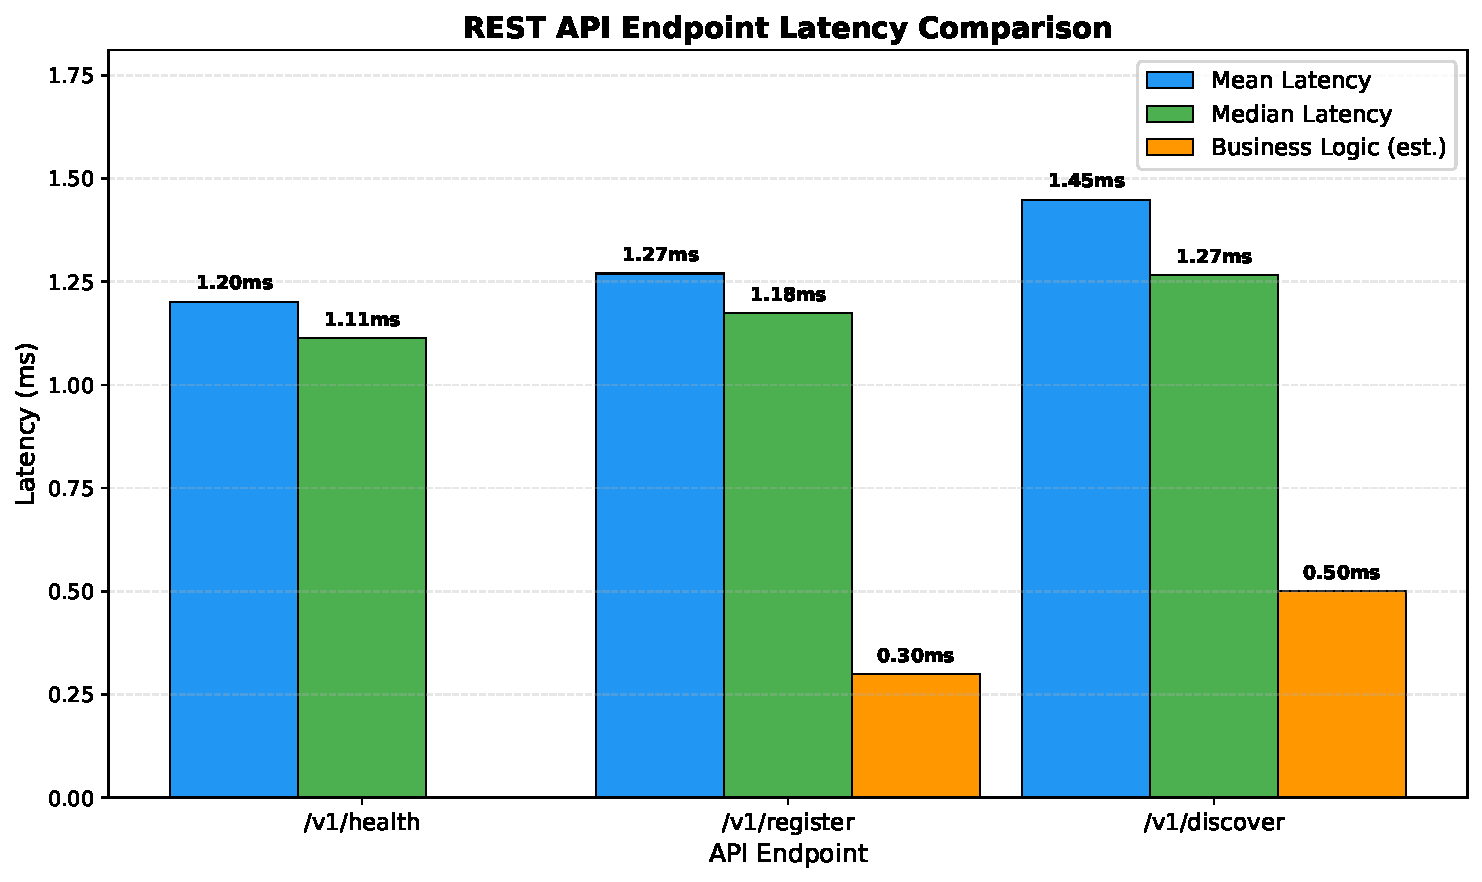
\includegraphics[width=0.85\columnwidth]{figures/api_bench.pdf}
\caption{REST API endpoint latency comparison. All endpoints respond in <1.5\textit{ms} including HTTP overhead.}
\label{fig:api-bench}
\end{figure}